%%%%%%%%%%%%%%%%%%%%%%%%%%%%%%%%%%%%%%%%%%%%%%%%%%%%%%%%%%
%%% Section 3: Modelling Reactive
%%%%%%%%%%%%%%%%%%%%%%%%%%%%%%%%%%%%%%%%%%%%%%%%%%%%%%%%%%

\section{Reactive ICS Modelling} \label{section:model}

% The goal of this model is to facilitate making design decisions when deploying intermittent computing devices in real-world environments by enabling designers to observe how the sizes of energy harvester and energy storage have an impact on the key design specifications, i.e. forward progress, dimensions, and interruption periods.

% We then illustrate a formulation which describes the relationship between forward progress and energy storage capacitance given different harvested power level in reactive intermittent computing as a part of the exploration model. 

% Assumptions. low variation in harvested power, how low? what's the impact of high variance input?
% given a constant current supply
To facilitate the understanding and exploration of reactive ICSs, we present a model which outputs the normalized forward progress $\alpha_{exe}$ when powered from a constant current supply $I_{harv}$. Parameters of this model are listed in Table~\ref{tab:parameter}. 
%This accounts for the \textit{Energy Storage} and \textit{Intermittent Load} modules in the system model, allowing the expected forward progress to be evaluated.
% The input parameters $I_{harv}$ and $C$ are related to the size configuration of energy harvester and energy storage respectively. 
% for a period of time that long enough to omit an individual uncompleted operating cycle. 
The model assumes that all configuration parameters remain constant. 

\begin{table}[!t]
    \renewcommand{\arraystretch}{1.2}
    \centering
    \caption{Model parameters of reactive ICS} 
    \label{tab:parameter}
    % Some packages, such as MDW tools, offer better commands for making tables
    % than the plain LaTeX2e tabular which is used here.
    \begin{tabular}{|c|c|}
        % \hline
        % \textbf{Parameter} & \textbf{Description} \\
        \hline
        \multicolumn{2}{|c|}{\textbf{Input Parameters}}\\
        \hline
        $I_{harv}$ & Energy harvester current supply\\
        $C$ & Energy storage capacitance\\
        \hline
        \multicolumn{2}{|c|}{\textbf{Configuration Parameters}}\\
        \hline
        $I_{exe}$ & Execution current draw\\
        $I_{lpm}$ & Low-power mode current draw\\
        %$I_{load}$ & Total current draw of load\\
        $I_{r}$ & Restore current draw\\
        $I_{s}$ & Save current draw\\
        $I_{leak}$ & Leakage current draw\\
        $V_{r}$ & Restore voltage threshold\\
        $V_{s}$ & Save voltage threshold\\
        $T_{r}$ & Restore time overhead\\
        $T_{s}$ & Save time overhead\\
        \hline
        \multicolumn{2}{|c|}{\textbf{Output Parameter}}\\
        \hline
        $\alpha_{exe}$ & Normalized forward progress \\ 
        \hline
    \end{tabular}
\end{table}

% Since supply current $I_{harv}$ and leakage current $I_{leak}$ constantly exist (though could be zero), 
For brevity, $I_{in}$ denotes the usable input current as expressed in (\ref{eq:in}). The effect of capacitor leakage current, $I_{leak}$, is discussed at the end of Section~\ref{subsec:formulation}.
\begin{equation}
  I_{in} = I_{harv} - I_{leak}
  \label{eq:in}
\end{equation}

\subsection{Operating Modes of Reactive ICS}

The behavior of reactive ICSs can be classified into three operating modes depending on the supply current, as shown in \figurename{~\ref{fig:operatingModes}}. These are differentiated by the relationship between input current $I_{in}$ and the system's current draw in its low-power mode (LPM) or active modes, i.e. $I_{lpm}$ and $I_{exe}$. We define the three modes as:

\begin{figure}[!t]
  \centering
  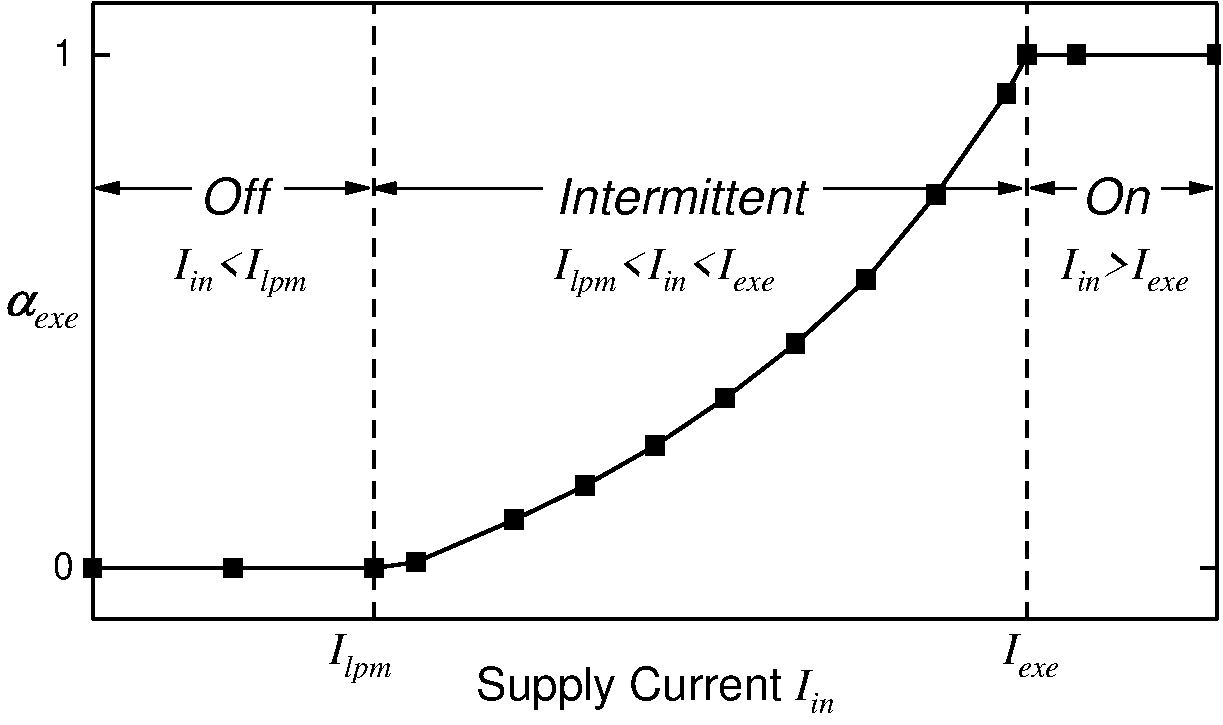
\includegraphics[width=3.2in]{OperatingMode0Fig.pdf}
  \caption{Operating modes of reactive ICSs, and achieved forward progress against supply current.}
  \label{fig:operatingModes}
\end{figure}

\begin{itemize}
	\item \textit{Off} mode: When $I_{in} < I_{lpm}$, the system stays inactive. The supply voltage $V_{cc}$ cannot rise above the restore threshold $V_{r}$ to wake the system and start execution. The LPM current $I_{lpm}$ includes the consumption of voltage monitoring circuits and system idle current.
	% Here, $I_{lpm}$ is induced after $V_{cc}$ goes above the minimum operating voltage $V_{off}$ where the system waits for $V_{cc}$ to reach $V_{r}$ (when $V_{off} < V_{cc} < V_{R}$). 

    \item \textit{On} mode: When $I_{in} > I_{exe}$, the system executes constantly as the supply voltage $V_{cc}$ never drops below $V_{s}$. $V_{cc}$ grows until $I_{in}$ and $I_{exe}$ are in equilibrium, which may result from $I_{in}$ decreasing due to poor impedance matching, or $I_{exe}$ increasing due to either greater current draw at higher voltage or dissipation through overvoltage protection circuits. 

	\item \textit{Intermittent} mode: When $I_{lpm} < I_{in} < I_{exe}$, the system executes intermittently after $V_{cc} > V_{r}$ and before $V_{cc} < V_{s}$. $V_{cc}$ can rise above $V_{r}$ and the system starts execution. However, the stored energy is then consumed by the load as $I_{in} < I_{exe}$, causing $V_{cc}$ to eventually drop below the save threshold $V_{s}$, where the system saves its state and enters LPM. The system stays in LPM until $V_{cc}$ rises to $V_{r}$ again and then resumes execution. 
	% In this mode, $V_{cc}$ oscillates approximately between $V_{r}$ and $V_{s}$, 'switching' on and off the execution. 
    In general, a higher $I_{in}$ leads to more forward progress in this mode, but the exact relationship between $I_{in}$ and forward progress requires further analysis.
    
	% The excess power either dissipates through circuits or overcharges $V_{cc}$. An overcharged $V_{cc}$ may affect harvesting efficiency due to poor impedance matching and reduce $I_{harv}$, such that current input and consumption are in equilibrium. 
	% In this model case, charging $V_{cc}$ above the maximum power point of the PV cell reduces $I_{harvest}$, and $V_{cc}$ is stable when $I_{harvest} = I_{exe} + I_{leak}$. 
\end{itemize}

\subsection{Formulating Forward Progress} \label{subsec:formulation}

Next, we derive formulations to calculate $\alpha_{exe}$ from $I_{in}$ and energy storage capacitance $C$. We then explore the effect of capacitor leakage on maximum forward progress. 

In the \textit{On} and \textit{Off} modes, the normalized forward progress is trivial to find (simply 1 and 0 respectively). In the \textit{Intermittent} mode,  as shown in \figurename{~\ref{fig:operatingCycle}}, the system goes through four intervals in turn, i.e. charging, restoring, executing, and saving, with current consumption of $I_{lpm}$, $I_{r}$, $I_{exe}$, and $I_{s}$ in each interval respectively. The normalized forward progress, i.e. effective execution time ratio, is indicated as $T_{exe} / T_{cycle}$, where $T_{exe}$ is the time spent on effective execution in one operating cycle and $T_{cycle}$ is the period of operating cycles. Hence, the forward progress given all supply levels is expressed as:
\begin{equation}
    \alpha_{exe} = \left\{
    \begin{aligned}
        & 0 & , & \quad \textit{Off} \, (I_{in} < I_{lpm}) \\
        & \frac{T_{exe}}{T_{cycle}} & , & \quad \textit{Intermittent} \, (I_{lpm} < I_{in} < I_{exe}) \\
        & 1 & , & \quad \textit{On} \, (I_{in} > I_{exe})
    \end{aligned}
    \right.
    \label{eq:feff}
\end{equation}

\begin{figure}[!t]
  \centering
  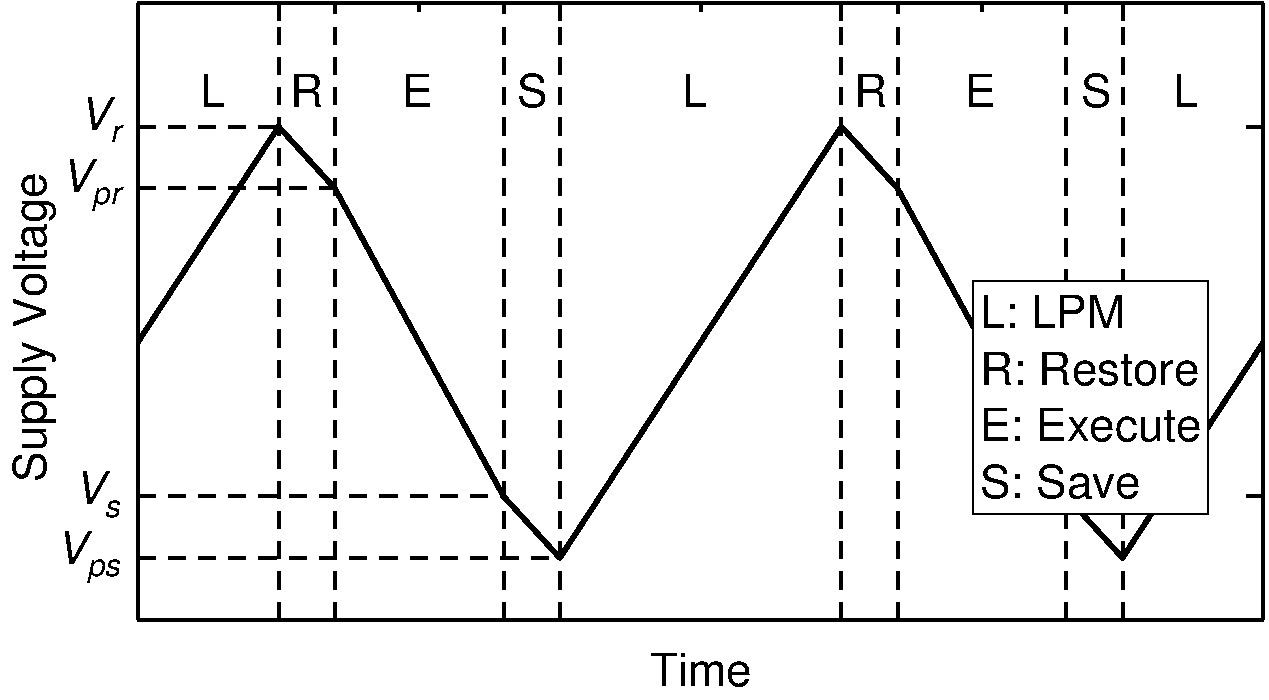
\includegraphics[width=3.33in]{CRESdemoFig}
  \caption{Operating cycles in the \textit{Intermittent} mode. }
  \label{fig:operatingCycle}
\end{figure}

In the following analysis, we focus on deriving $T_{exe} / T_{cycle}$ in the \textit{Intermittent} mode. Let $V_{pr}$ (post-restore) and $V_{ps}$ (post-save) denote the voltage after restoring and saving operations. $V_{pr}$ and $V_{ps}$ can be calculated as:
\begin{equation}
  V_{pr} = V_{r} + \frac{T_{r} (I_{in} - I_{r})}{C}
  \label{eq:vpr}
\end{equation}
\begin{equation}
  V_{ps} = V_{s} + \frac{T_{s} (I_{in} - I_{s})}{C}
  \label{eq:vps}
\end{equation}
With (\ref{eq:vpr}), the time spent on effective execution $T_{exe}$ in one operating cycle can be expressed as:
\begin{equation}
%   \begin{aligned}
    T_{exe} = \frac{C(V_{pr} - V_{s})}{I_{exe} - I_{in}} 
    % & = \frac{C(V_{r} - V_{s}) + T_{r} (I_{in} - I_{r})} {I_{exe} - I_{in}}
%   \end{aligned}
  \label{eq:texe}
\end{equation}
Analogously, with (\ref{eq:vps}), the charging interval can be described as:
\begin{equation}
%   \begin{aligned}
    T_{charge} = \frac{C(V_{r} - V_{ps})}{I_{in} - I_{lpm}}
    % & = \frac{C(V_{r} - V_{s}) - T_{s} (I_{in} - I_{s})} {I_{in} - I_{lpm}}
%   \end{aligned}
  \label{eq:tcharge}
\end{equation}
With (\ref{eq:texe}) and (\ref{eq:tcharge}), the period of an operating cycle is:
\begin{equation}
%   \begin{aligned}
    T_{cycle} = \quad T_{charge} + T_{r} + T_{exe} + T_{s} 
%     = & \quad \frac{C (V_{r} - V_{s}) + T_{s} (I_{s} - I_{lpm})}{I_{in} - I_{lpm}} \quad + \\
%     & \quad \frac{C (V_{r} - V_{s}) + T_{r} (I_{exe} - I_{r})}{I_{exe} - I_{in}}
%   \end{aligned}
  \label{eq:tperiod}
\end{equation}

Finally, combining (\ref{eq:vpr})--(\ref{eq:tperiod}), we obtain normalized forward progress $\alpha_{exe}$ in the \textit{Intermittent} mode as:
\begin{equation}
    \begin{aligned}
        \alpha_{exe} &= \frac{T_{exe}}{T_{cycle}} \\ %, \quad I_{lpm} < I_{in} < I_{exe}
                     &= \frac{\frac{C (V_{r} - V_{s}) + T_{r} (I_{in} - I_{r})} {I_{exe} - I_{in}}}{\quad \frac{C (V_{r} - V_{s}) + T_{s} (I_{s} - I_{lpm})}{I_{in} - I_{lpm}} + \frac{C (V_{r} - V_{s}) + T_{r} (I_{exe} - I_{r})}{I_{exe} - I_{in}}} \\
                    %  &= \frac{\scriptstyle \bigl[C (V_{r} - V_{s}) + T_{r} (I_{in} - I_{r}) \bigr] (I_{in} - I_{lpm})}{\scriptscriptstyle C (V_{r} - V_{s}) (I_{exe} - I_{lpm}) + T_{s} (I_{in} - I_{s}) (I_{exe} - I_{in}) + T_{r} (I_{exe} - I_{r}) (I_{in} - I_{lpm})} \\
    \end{aligned}
    \label{eq:texepercent}
\end{equation}
In the numerator $T_{exe}$, $C(V_{r} - V_{s})$ represents the amount of charge in the capacitor available for restoring and executing. $T_{r} (I_{in} - I_{r})$ represents the charge used by a restore operation. $I_{exe} - I_{in}$ is the rate of charge consumption from the energy storage during execution.

% \footnote{Calculation breakdowns of differential analysis is attached in Appendix.}
% Higher $\alpha_{exe}$ leads to more time spent on forward progress. 

% As $d\alpha_{exe} / dI_{in}$ is positive, higher harvested current $I_{harv}$ leads to more forward progress. 
To explore the effect of energy storage on forward progress, we need to analyze $d\alpha_{exe} / dC$. Here, if we assume that $I_{leak}$ remains constant, $\alpha_{exe}$ keeps increasing and approaches $(I_{in} - I_{lpm}) / (I_{exe} - I_{lpm})$ when energy storage capacitance $C$ increases. Defining $(I_{in} - I_{lpm}) / (I_{exe} - I_{lpm})$ as $\alpha_{exe\_ideal}$, $\alpha_{exe} = \alpha_{exe\_ideal}$ is an ideal case, where restore and save overheads are absent.

In an electrolytic capacitor, however, $I_{leak}$ typically increases with $C$ with the following relationship~\cite{avxleakage}:
\begin{equation}
    I_{leak} = kCV_{cc}
    \label{eq:ileak}
\end{equation}
where $k$ is a constant normally in a range 0.01 to 0.03 ($\frac{A}{F \cdot V}$). Combining (\ref{eq:ileak}) with (\ref{eq:in}), $dI_{in} / dC$ is $-kV_{cc}$, meaning $I_{in}$ decreases linearly as $C$ increases. Thus, when $C$ increases, $\alpha_{exe}$ keeps approaching $\alpha_{exe\_ideal}$ while $\alpha_{exe\_ideal}$ decreases. Hence, we believe that there is a capacitance value that leads to the maximum $\alpha_{exe}$ considering $I_{leak}$ increases with $C$.
% \cite{alcapacitor}
% Also, the time overhead of state saving and restoring operations $T_{RS\%}$ can be calculated as:
% \begin{equation}
%   T_{RS\%} = \frac{T_{R} + T_{S}}{T_{exe} + T_{R} + T_{S}}
% \end{equation}


% In Equation~(\ref{eq:feff}), we get the relationship between forward progress and the sizes of energy harvester and energy storage. 
